\normaltrue \difficilefalse \tdifficilefalse
\correctionfalse

%\UPSTIidClasse{11} % 11 sup, 12 spé
%\newcommand{\UPSTIidClasse}{12}
% ATS 2019
\exer{Le banc balafre $\star$ \label{B2:22:50}}
\setcounter{numques}{0}
\UPSTIcompetence[2]{B2-22}
\index{Compétence B2-22}
\index{Le Banc Balafre}
\index{Moteur asynchrone}
\index{MAS}
\ifcorrection
\else
\textbf{Pas de corrigé pour cet exercice.}
\fi

\ifprof
\else



\begin{obj}
L'objectif est de valider les exigences suivantes.
\begin{itemize}
\item 1.01 -- Couple résistant : le couple résistant exercé par le film d’eau sur le joint (rotor) à $\SI{6000}{tr.min^{-1}}$  est estimé à $C_{\text{res}} = \SI{300}{Nm}$.
\item 1.02 -- Vitesse de rotation : la vitesse cible NC (vitesse de rotation du rotor de joint) doit
pouvoir être réglée à une valeur choisie entre \SI{5000}{tr.min^{-1}} 
et \SI{7000}{tr.min^{-1}}.
\item 1.03 -- Loi de commande : la mise en rotation doit se faire à accélération constante pendant une durée n’excédant par $T_{\text{acc}} = \SI{5}{s}$.
\end{itemize}

Nous allons modéliser le moteur asynchrone Leroy Somer
PLS-280-MP. Ceci va nous permettre de déterminer sa caractéristique de couple. Cette
caractéristique sera utilisée dans les parties suivantes et nous permettra dans cette partie
de déterminer la fréquence de commande du moteur pour la phase de mesure en régime
stationnaire.
\end{obj}


Données et hypothèses :
\begin{itemize}
\item le réseau d’alimentation électrique fournit une tension 230/\SI{400}{V} en \SI{50}{Hz} ;
\item la plaque signalétique du moteur est donnée en figure \autoref{fig_50_01} ;
\item on négligera les pertes fer et les pertes mécaniques dans le moteur ;
\item les pertes Joule statoriques sont également négligées.
\end{itemize}

\begin{figure}[H]
\centering
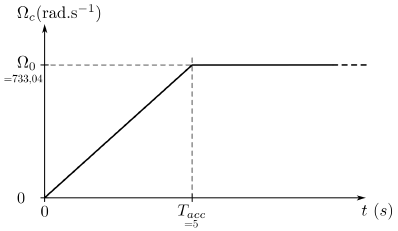
\includegraphics[width=\linewidth]{fig_50_01}
\caption{Plaque signalétique du moteur PLS-280-MP \label{fig_50_01}}
\end{figure}
\fi

\question{En utilisant les informations de la plaque signalétique, montrer que le
moteur possède $p = 1$ paire de pôles.}
\ifprof
\else
\fi

\question{À partir de la plaque signalétique, en détaillant les calculs, déterminer
le glissement en fonctionnement nominal $g_N$ ainsi que le couple utile nominal $C_{uN}$.}
\ifprof
\else
\fi

On donne sur la figure \autoref{fig_50_02} le modèle équivalent ramené au stator d’une phase du moteur.
$L_0$ représente l’inductance de magnétisation et $L_c$ l’inductance des fuites totales d’une
phase (rotorique ramenée au stator et stator). On note $g$ le glissement. On rappelle que la
puissance dissipée dans la résistance $R/g$ correspond à la puissance transmise du stator
au rotor. Cette puissance peut être décomposée en une résistance $R$ correspondant aux
pertes Joule dans le rotor en série avec une résistance $R(1 - g)/g$ correspondant à la
puissance électromécanique fournie au rotor.

\begin{rem}
Ce modèle est celui du bobinage couplé en triangle. La tension $\underline{U_S}$ représente
la tension entre phases, c’est-à-dire, vue de l’extérieur, la tension composée de valeur
nominale \SI{400}{V}. Le courant $\underline{i_S}$ représente le courant dans chaque phase statorique. La
notation conventionnelle $\underline{j_S}$ pour ce courant n’est pas utilisée ici pour éviter toute confusion
avec les notations des nombres complexes.
\end{rem}

\begin{figure}[H]
\centering
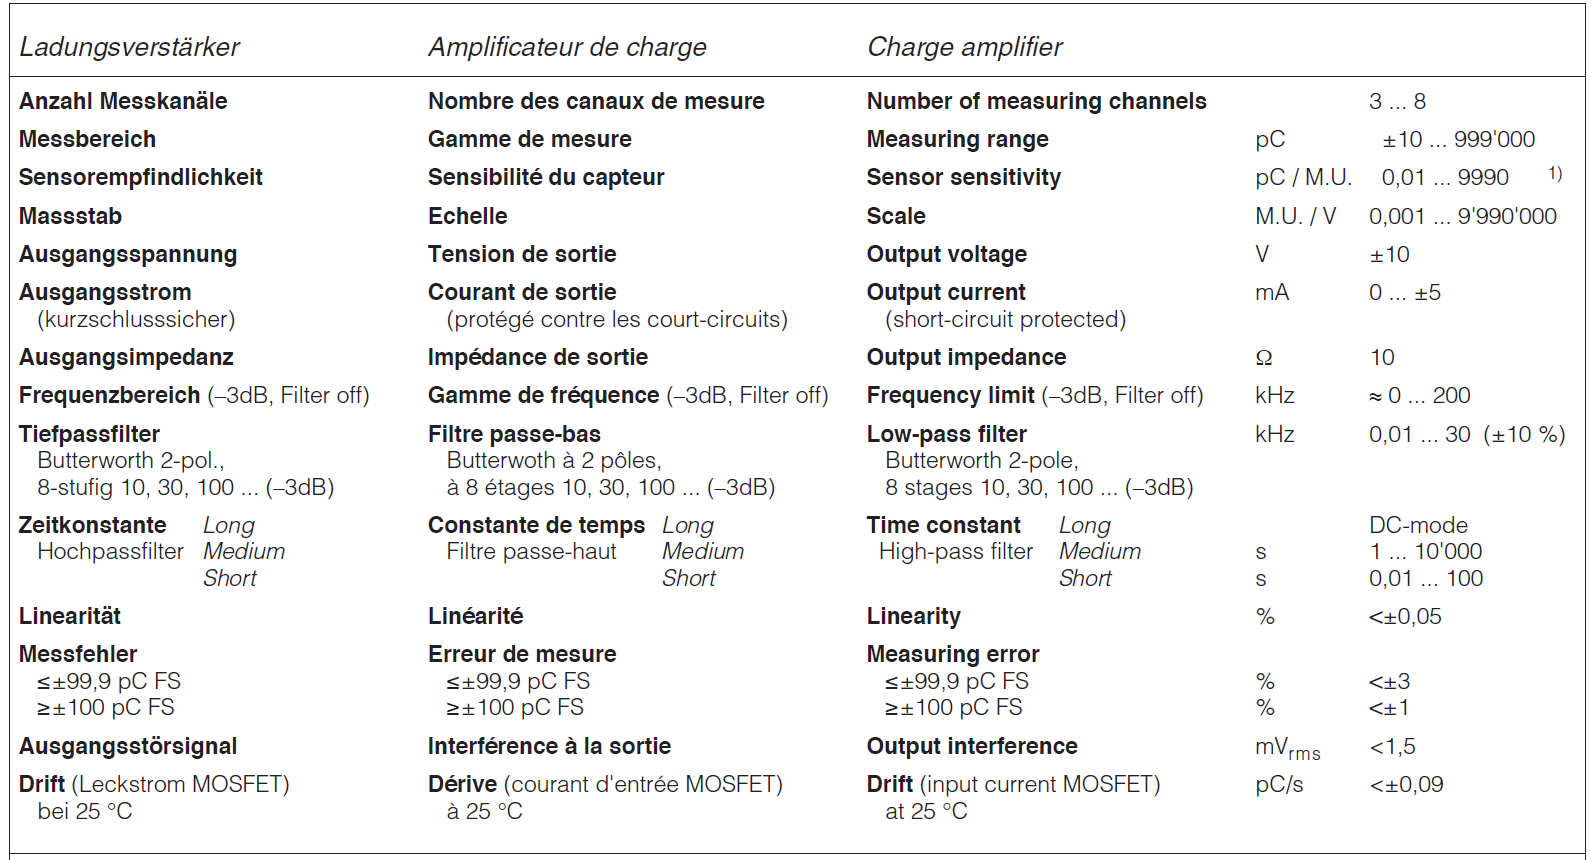
\includegraphics[width=\linewidth]{fig_50_02}
\caption{Modèle équivalent ramené au stator d’une phase du moteur \label{fig_50_02}}
\end{figure}

\question{Exprimer la puissance électromécanique $P_{EM}$ fournie au rotor en fonction
de $U_S$ (valeur efficace de la tension $\underline{U_S}$), de la résistance $R$, du glissement $g$ de l’inductance
$L_c$ et de la pulsation d’alimentation $\omega$ du moteur.}
\ifprof
\else
\fi


\question{Exprimer la puissance électromécanique $P_{EM}$ en fonction du couple
électromagnétique $C_{EM}$ et de la vitesse de rotation $\Omega$ de l’arbre moteur.}
\ifprof
\else
\fi

\question{Exprimer la vitesse de rotation $\Omega$ de l’arbre en fonction du glissement $g$
et de la vitesse de synchronisme $\Omega_S$. En déduire l’expression du couple électromagnétique
$C_{EM}$ en fonction de $U_S^2$, $\omega$, $g$, $R$, $L_c$, et $p$ (le nombre de paires de pôles par phase).}
\ifprof
\else
\fi

\question{En précisant bien vos hypothèses, justifier que l’expression du couple
utile disponible sur l’arbre moteur est $C_u = \dfrac{3pU_S^2}{\omega}\cdot\dfrac{\dfrac{R}{g}}{\left(\dfrac{R}{g}\right)^2+\left(L_c\omega\right)^2}$.}
\ifprof
\else
\fi

À l’aide de cette équation, on obtient la figure \autoref{fig_50_03} qui représente l’allure de la courbe de
couple en fonction de la vitesse de rotation $N$ de l’arbre moteur.

\begin{figure}[H]
\centering
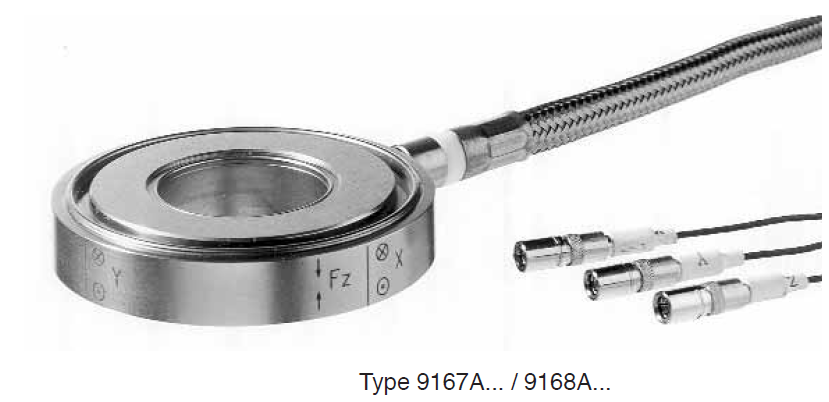
\includegraphics[width=\linewidth]{fig_50_03}
\caption{Allure de la courbe de couple utile du moteur en fonction de la vitesse de
rotation de l’arbre \label{fig_50_03}}
\end{figure}

\question{À l’aide des points A, B, C et D, identifier sur cette courbe 
%\begin{itemize}
%\item 
le point de fonctionnement nominal,
%\item 
le démarrage du moteur,
%\item 
le point de synchronisme,
%\item  
la zone de fonctionnement instable du moteur.}
%\end{itemize}
\ifprof
\else
\fi


Le constructeur précise le rapport du couple maximal sur couple nominal : $C_M/C_N = 3,5$.
On rappelle que le couple utile est maximal pour une valeur du glissement telle que
$R/g = L_c\omega$.

\question{En déduire l’expression de $L_c$ en fonction de $p$, $U_S$, $C_M$ et $\omega$ et faire
l’application numérique.}
\ifprof
\else
\fi

\question{Que peut-on dire de $R/g$ par rapport à $L_c\omega$ au voisinage du point de
fonctionnement nominal ? En déduire l’expression de $R$ en fonction du couple nominal
$C_N$, du glissement nominal $g_N$, de $p$, $U_S$ et de $\omega$.}
\ifprof
\else
\fi

\begin{rem}
On fera l’application numérique en prenant $g_N = 1,4 \times 10^{-2}$ et $C_N =\SI{213}{Nm}$.
\end{rem}

Le variateur utilisé pour la commande du moteur fonctionne en $U_S/f$ constant. À l’aide
des valeurs calculées précédemment, on a tracé sur la figure \autoref{fig_50_04}  les courbes de couple utile
en fonction de la vitesse de rotation pour différentes valeurs de fréquence de commande.

\begin{figure}[H]
\centering
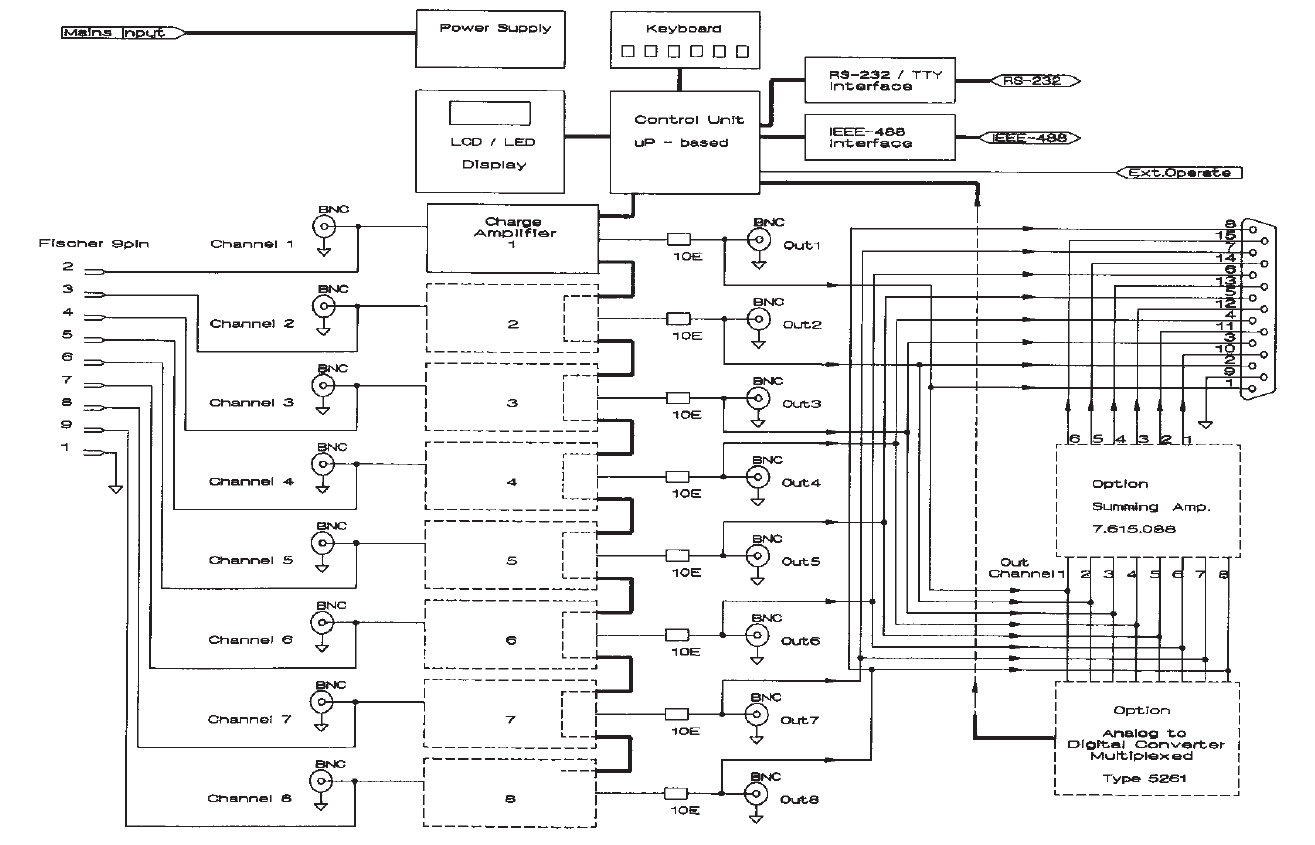
\includegraphics[width=\linewidth]{fig_50_04}

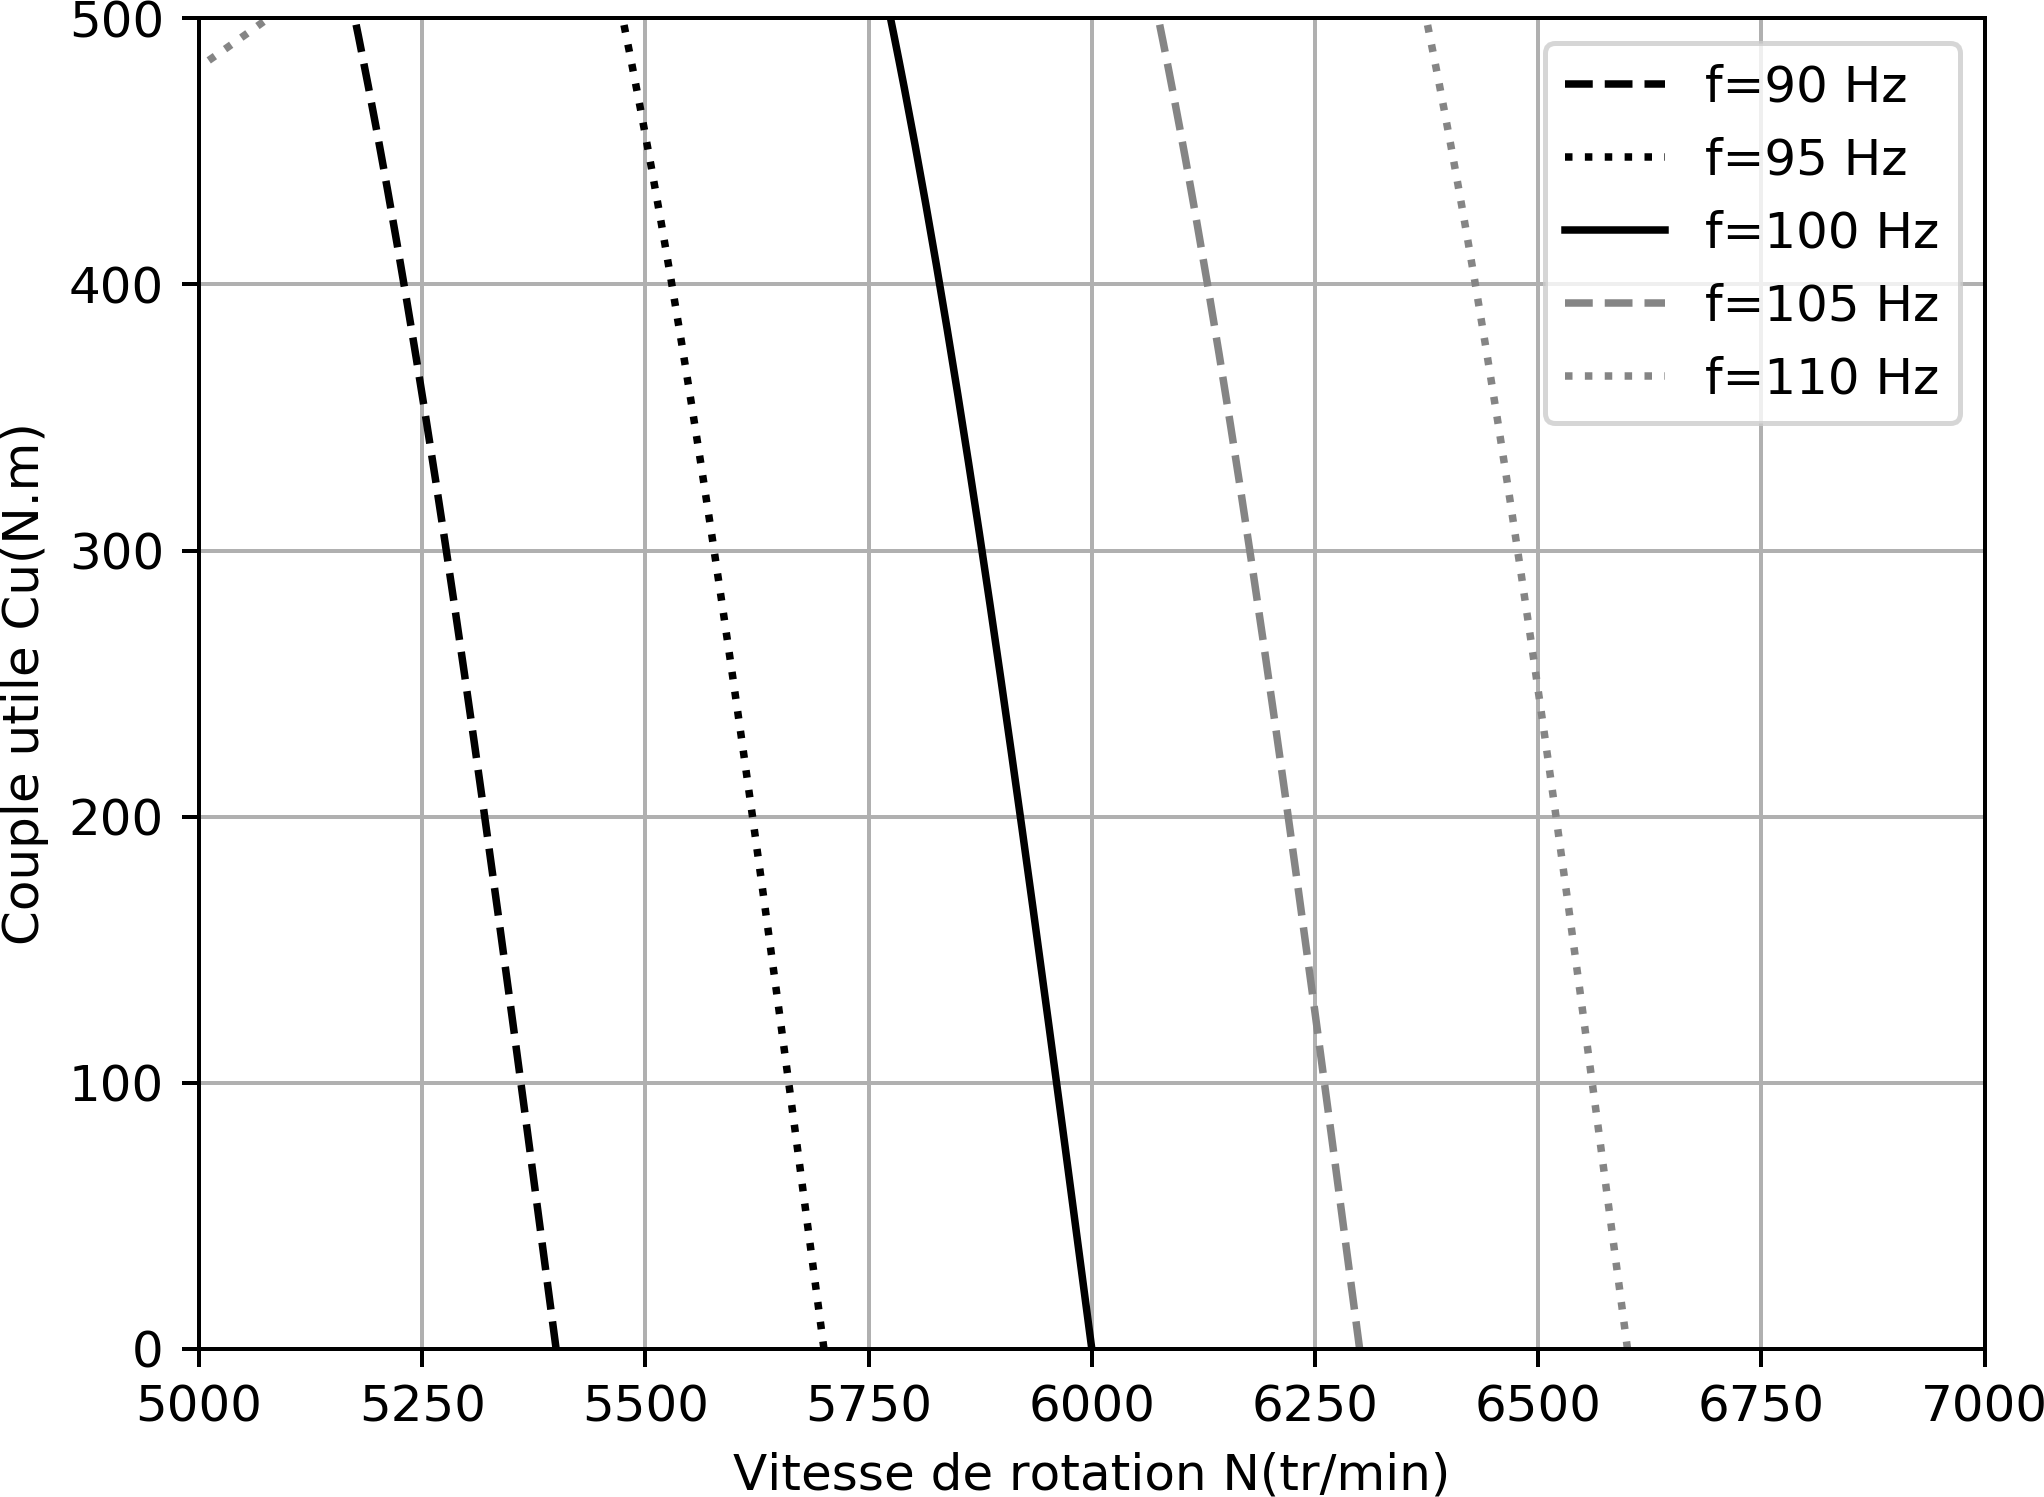
\includegraphics[width=\linewidth]{fig_50_05}
\caption{Évolution du couple utile en fonction de la vitesse de rotation pour des
fréquences de commande de \SI{90}{Hz} à \SI{110}{Hz}. \label{fig_50_04}}
\end{figure}

\question{Déterminer quelle fréquence doit être imposée
par le variateur pour maintenir une vitesse de \SI{6000}{tr.min^{-1}} en présence d’un couple
résistant correspondant au couple $C_{\text{res}} = \SI{300}{Nm}$ défini par l’exigence 1.01 du cahier des
charges.}
\ifprof
\else
\fi

\ifprof
\else
\begin{flushright}
\footnotesize{Corrigé  voir \ref{B2:22:50}.}
\end{flushright}%
\fi